\begin{frame}{Talk outline}
\protect\hypertarget{talk-outline}{}

\begin{itemize}
\tightlist
\item
  What is streaming data?
\item
  Computational models for streaming data
\item
  Statistical models for streaming data
\item
  An example: nowcasting urban rainfall events
\end{itemize}
\bigskip

Joint work with: Andy Golightly, Naomi Hannaford, Sarah Heaps, Yuanzhi Huang, Stephen Johnson, Kevin Wilson, \ldots

\bigskip

Fuding from UKRI-NERC and The Alan Turing Institute

\end{frame}

\begin{frame}{Streaming data applications}
\protect\hypertarget{streaming-data-applications}{}

\begin{itemize}
\tightlist
\item
  Streaming voice and video applications

  \begin{itemize}
  \tightlist
  \item
    Zoom, Netflix, YouTube, Spotify, etc.
  \item
    Typically streamed directly \emph{over the internet} to your display
  \item
    Even if the video is downloaded to local storage, it is still
    \emph{streamed} from storage and decompressed on-the-fly for
    real-time viewing - the entire video is never fully decompressed in
    RAM - not just about moving data over the internet
  \end{itemize}
\item
  Real-time financial market trading data

  \begin{itemize}
  \tightlist
  \item
    Automated trading systems
  \item
    Decision support for human traders
  \end{itemize}
\item
  On-line processing (and compression) of scientific experiments

  \begin{itemize}
  \tightlist
  \item
    Biological sequencing technologies, neuroscience data
  \item
    Collider experiments, astronomical surveys
  \end{itemize}
\item
  Real time sensor network data for continuous monitoring

  \begin{itemize}
  \tightlist
  \item
    Traffic (and pollution) monitoring, weather forecasting, healthcare
    wearables, \ldots{}
  \end{itemize}
\end{itemize}

\end{frame}

\begin{comment}

\begin{frame}{Turing Fellow project}
\protect\hypertarget{turing-fellow-project}{}

\begin{block}{Streaming data modelling for real-time monitoring and
forecasting}

\begin{itemize}
\item
  Computational architecture and infrastructure
\item
  Statistical methodology and algorithms
\item
  Case studies: Urban Analytics (The Urban Observatory - eg. air
  pollution), Healthcare (neuroscience), engineering biology, \ldots{}
\end{itemize}

\emph{Joint work with A Golightly, S Heaps, Y Huang, N Hannaford, A
Hardy, \ldots{}}

\end{block}

\end{frame}


\end{comment}


\begin{frame}{Streaming data architecture}
\protect\hypertarget{streaming-data-architecture}{}

\begin{block}{Fundamental concepts}

\begin{itemize}
\tightlist
\item
  A \emph{stream} is a (possibly infinite) sequence of values of a given
  (potentially complex) data type, with a definite order
\item
  The stream is accessed one value at a time, and processing is done
  incrementally, triggered by the arrival of each value
\item
  Typically only \emph{one pass} over the data is possible
\item
  Streams are connected together in a DAG called the \emph{flow graph}
\end{itemize}

\end{block}

\begin{block}{Software libraries and frameworks}

\begin{itemize}
\tightlist
\item
  \emph{Storm}, \emph{Heron}, \emph{Spark streaming}, \emph{Akka
  streams}, \emph{Flink}, \emph{Kafka streams} are well-known examples
  of streaming data frameworks
\item
  Frameworks are often run on the \emph{JVM}, built in languages with
  good support for \textbf{functional programming} (FP), such as
  \emph{Scala}, and rely to a greater-or-lesser extent on FP principles
  such as \emph{functional reactive programming} (FRP)
\end{itemize}

\end{block}

\end{frame}

\begin{frame}[fragile]{Functional models of streaming data}
\protect\hypertarget{functional-models-of-streaming-data}{}

\begin{itemize}
\tightlist
\item
  A key streaming data processing abstraction is a pure
  \textbf{function}:
  \[h: \mathcal{X} \times \mathcal{Y} \longrightarrow \mathcal{X}\]
\end{itemize}

\begin{Shaded}
\begin{Highlighting}[]
\NormalTok{advance: (State, Observation) => State}
\end{Highlighting}
\end{Shaded}

combining current world knowledge (encapsulated in a \texttt{State})
together with the latest observation to get an updated world view

\begin{itemize}
\tightlist
\item
  Then given
  \(x_0\in\mathcal{X},\quad \mathbf{y} \in \mathcal{Y}^{\mathbb{N}}\)
\end{itemize}

\begin{Shaded}
\begin{Highlighting}[]
\NormalTok{s0: State, sObs: Stream[Observation]}
\end{Highlighting}
\end{Shaded}

we transform the stream of observations \(\mathbf{y}\) to states
\(\mathbf{x}\in\mathcal{X}^{\mathbb{N}}\):

\begin{Shaded}
\begin{Highlighting}[]
\NormalTok{sState: Stream[State] = sObs.}\FunctionTok{scan}\NormalTok{(s0)(advance)}
\end{Highlighting}
\end{Shaded}

via successive application of \(h\).

\end{frame}

\begin{frame}[fragile]{Stream transformation}
\protect\hypertarget{stream-transformation}{}

Streams are \emph{functors}, since they \texttt{map}:

\begin{Shaded}
\begin{Highlighting}[]
\NormalTok{  Stream[A].}\FunctionTok{map}\NormalTok{[B](f: A => B): Stream[B]}
\end{Highlighting}
\end{Shaded}

The \texttt{scan} operation, sometimes called \texttt{scanLeft}, has
signature:

\begin{Shaded}
\begin{Highlighting}[]
\NormalTok{  scanLeft[B](init: B)(advance: (B, A) => B): Stream[B]}
\end{Highlighting}
\end{Shaded}

For example:

\begin{Shaded}
\begin{Highlighting}[]
\KeywordTok{val}\NormalTok{ naturals = Stream.}\FunctionTok{iterate}\NormalTok{(}\DecValTok{1}\NormalTok{)(_ + }\DecValTok{1}\NormalTok{)}
\CommentTok{// 1, 2, 3, 4, ...}
\KeywordTok{val}\NormalTok{ evens = naturals }\FunctionTok{map}\NormalTok{ (_ * }\DecValTok{2}\NormalTok{)}
\CommentTok{// 2, 4, 6, 8, ...}
\KeywordTok{val}\NormalTok{ triangular = naturals.}\FunctionTok{scan}\NormalTok{(}\DecValTok{0}\NormalTok{)(_ + _).}\FunctionTok{drop}\NormalTok{(}\DecValTok{1}\NormalTok{)}
\CommentTok{// 1, 3, 6, 10, ...}
\end{Highlighting}
\end{Shaded}

\end{frame}

\begin{frame}[fragile]{State-space modelling}
\protect\hypertarget{state-space-modelling}{}

In state-space modelling, we have a

\begin{itemize}
\tightlist
\item
  forward model: \(X_t | x_{t-1} \sim f(x_t|x_{t-1})\) or
  \texttt{f:\ X\ =\textgreater{}\ P{[}X{]}}
\item
  and observation model: \(Y_t|x_t \sim g(y_t|x_t)\) or
  \texttt{g:\ X\ =\textgreater{}\ P{[}Y{]}}
\end{itemize}

where \texttt{P{[}\_{]}} is a suitable \emph{probability monad}, and
\(f\), \(g\) are \emph{Markov kernels}.

For \emph{filtering} we typically think in terms of predict-update
steps:

\begin{itemize}
\tightlist
\item
  \(p(x_{t-1}|\mathcal{Y}_{t-1}) \rightarrow p(x_t|\mathcal{Y}_{t-1})\)
  or \texttt{predict:\ P{[}X{]}\ =\textgreater{}\ P{[}X{]}}
\item
  \(p(x_t|\mathcal{Y}_{t-1}) \rightarrow p(x_t|\mathcal{Y}_t)\) or
  \texttt{update:\ (P{[}X{]},Y)\ =\textgreater{}\ P{[}X{]}}
\end{itemize}

\texttt{predict} is monadic \texttt{flatMap} (or
\texttt{\textgreater{}\textgreater{}=}) with \texttt{f}, and
\texttt{update} is \emph{probabilistic conditioning} (Bayesian updating)
via \texttt{g}

Streaming:
\texttt{advance\ =\ update\ compose\ predict\textquotesingle{}} where
\texttt{State\ =\ P{[}X{]}} - eg. one step of a Kalman or particle
filter

\end{frame}

\begin{frame}{Composable functional models of on-line algorithms and
PPLs}
\protect\hypertarget{composable-functional-models-of-on-line-algorithms-and-ppls}{}

\begin{itemize}
\item
  Once we start to think about filtering in terms of operations
  involving probability monads and Markov kernels, it becomes easier to
  think about how to make models and algorithms composable and scalable,
  and about the connection to \emph{probabilistic programming} and
  monadic \emph{probabilistic programming languages} (PPLs)
\item
  Possible to think about all of the standard models and algorithms for
  SSMs within this framework: Kalman filters (regular, extended,
  unscented, ensemble, \ldots{}), particle filters (bootstrap, SIR,
  auxiliary, \ldots{}), etc.
\end{itemize}

\textbf{Law, W (2019)} Functional probabilistic programming for scalable
Bayesian modelling, \emph{arXiv}, 1908.02062

\end{frame}

\begin{frame}{POMP models}
\protect\hypertarget{pomp-models}{}

\begin{itemize}
\tightlist
\item
  Classical SSMs assume that the data are on a regular equispaced time
  grid, so that the state evolution model \(f(x_t|x_{t-1},\theta)\)
  represents a single time step of the process
\item
  Many sensors and devices do not generate data on a regular grid,
  either by design, or due to crashes/reboots creating large gaps of
  missing values, pushing observations onto a \emph{misaligned grid}, or
  changes in sampling frequency, etc.
\item
  \textbf{Partially observed Markov process} (POMP) models generalise
  classical SSMs in two important ways:

  \begin{itemize}
  \tightlist
  \item
    The state evolution model formulated in \emph{continuous time}, and
    is described by a transition kernel \(f(x_{t+t'}|x_t,t',\theta)\)
  \item
    It is not (necessarily) required that the transition kernel can be
    \emph{evaluated} --- only that the state process can be
    stochastically \emph{simulated} forwards in time
  \end{itemize}
\end{itemize}

\end{frame}

\begin{frame}{On-line filtering of POMP models}
\protect\hypertarget{on-line-filtering-of-pomp-models}{}

\begin{itemize}
\tightlist
\item
  The ``bootstrap'' particle filter is a ``likelihood free'' algorithm
  for sequentially computing the filtering distribution of a POMP model
  (for fixed \(\theta\)): \[
  \pi(x_t|\mathcal{Y}_t),\ \text{ where } \mathcal{Y}_t \equiv \{y_s|y_s\in\mathcal{Y},s\leq t\}
  \]
\item
  Although it is typically presented in discrete time, it works fine for
  continuous time processes observed discretely at irregular times
\item
  Additionally, composable (and tractable) families of continuous time
  transition kernels can be built using similar techniques as are
  sometimes used for discrete time DLMs
\end{itemize}

\textbf{Law \& W (2018)}
\href{https://doi.org/10.1007/s11222-017-9783-1}{Composable models for
online Bayesian analysis of streaming data}, \emph{Statistics and
Computing}, \textbf{28}:1119-37.

\end{frame}

\begin{frame}{What makes an algorithm ``on-line''?}
\protect\hypertarget{what-makes-an-algorithm-on-line}{}

\begin{itemize}
\tightlist
\item
  Not all streaming data applications are about time series
\item
  Many are just about analysing data based on a single pass
\item
  Almost any statistical algorithm can be expressed in the form of a
  streaming data algorithm
\item
  All of the data observed so far can be embedded in the \emph{state},
  and any analysis whatsoever of the data can be restarted from scratch
  with the arrival of each new observation!
\item
  We wouldn't consider such an analysis to be \emph{genuinely} on-line
\item
  We typically assume that the ``size'' of the state is bounded, and
  that the computational ``complexity'' of the \emph{advance} step has
  bounded expectation
\end{itemize}

\end{frame}

\begin{frame}{Spatio-temporal modelling}
\protect\hypertarget{spatio-temporal-modelling}{}

\begin{block}{Spatio-temporal SSMs}

\begin{itemize}
\tightlist
\item
  SSMs/POMPs fit naturally into the streaming data framework
\item
  Can be ``on-line'', since the \textbf{Markov property} for the hidden
  state process facilitates the bounding of state size and computation
  associated with updating
\end{itemize}

\end{block}

\begin{block}{Spatio-temporal GPs}

\begin{itemize}
\tightlist
\item
  Relatively straightforward to formulate GPs sequentially and embed in
  a streaming data framework
\item
  Most commonly used space-time covariance functions don't lead to
  simple Markov properties, so special techniques for ``scalable'' and
  ``streaming'' GPs must be used to ensure the algorithms are genuinely
  ``on-line''
\end{itemize}

\end{block}

\end{frame}

\begin{comment}

\begin{frame}{Scalable GP modelling}
\protect\hypertarget{scalable-gp-modelling}{}

\begin{itemize}
\tightlist
\item
  As the number of observations, \(n\), grows, the \(n\times n\)
  covariance (or precision) matrix gradually becomes problematic
  (whether inversion is explicit or not)
\item
  Can subset or merge design points in more-or-less principled ways, or
  form some other sparse or low-rank approximation of the covariance (or
  precision) matrix
\item
  There is also interest in learning GP hyper-parameters (such as length
  scales) in an on-line fashion
\item
  Hybrid approaches using off-line algorithms for learning static
  (hyper)parameters and on-line algorithms for dynamic state work well
  in practice
\item
  Very active research area
\end{itemize}

\end{frame}

\begin{frame}[fragile]{Example application: pollution monitoring}
\protect\hypertarget{example-application-pollution-monitoring}{}

\begin{block}{The Urban Observatory: \texttt{urbanobservatory.ac.uk}}

\begin{itemize}
\tightlist
\item
  The largest set of publicly available real time urban data in the UK
  --- web API (and also a \emph{websocket} for real time data)
\item
  eg. Temperature, rainfall and air quality sensors around the city
\item
  Rainfall radar data
\item
  \emph{Multivariate}, \emph{spatial}, \emph{temporal},
  \emph{irregularly observed}, \emph{mixed modality} (eg. point and
  areal)
\end{itemize}

\end{block}

\begin{block}{Pollution mapping in real time}

\begin{itemize}
\tightlist
\item
  Pollution monitors at various (fixed) locations around the city
\item
  Measurements every few minutes from every sensor, but not on a fixed
  grid, and not temporally aligned across sensors
\item
  Would like to ``nowcast'' a spatially continuous map of pollution
  levels across the city, updated with each new observation
\end{itemize}

\end{block}

\end{frame}

\begin{frame}{Pollution monitoring application}
\protect\hypertarget{pollution-monitoring-application}{}

\begin{itemize}
\tightlist
\item
  Urban observatory provides APIs (and a websocket) for accessing
  multiple air pollution measurements (eg. CO, NO2, NO, O3, PM1, PM4,
  PM10, PM25)
\item
  New small stream processing application server (in Scala), consuming a
  live stream of pollution measurements from an array of sensors around
  the city, updating a spatio-temporal GP in real-time, generating a new
  stream containing a now-casting pollution map (with uncertainty), for
  consumption by a small web front-end visualisation application (in JS)
\item
  Front-end application consumes nowcast map stream (via a websocket)
  and renders in a web page
\end{itemize}

\end{frame}

\begin{frame}{Pollution nowcasting}
\protect\hypertarget{pollution-nowcasting}{}

\begin{figure}
\centering
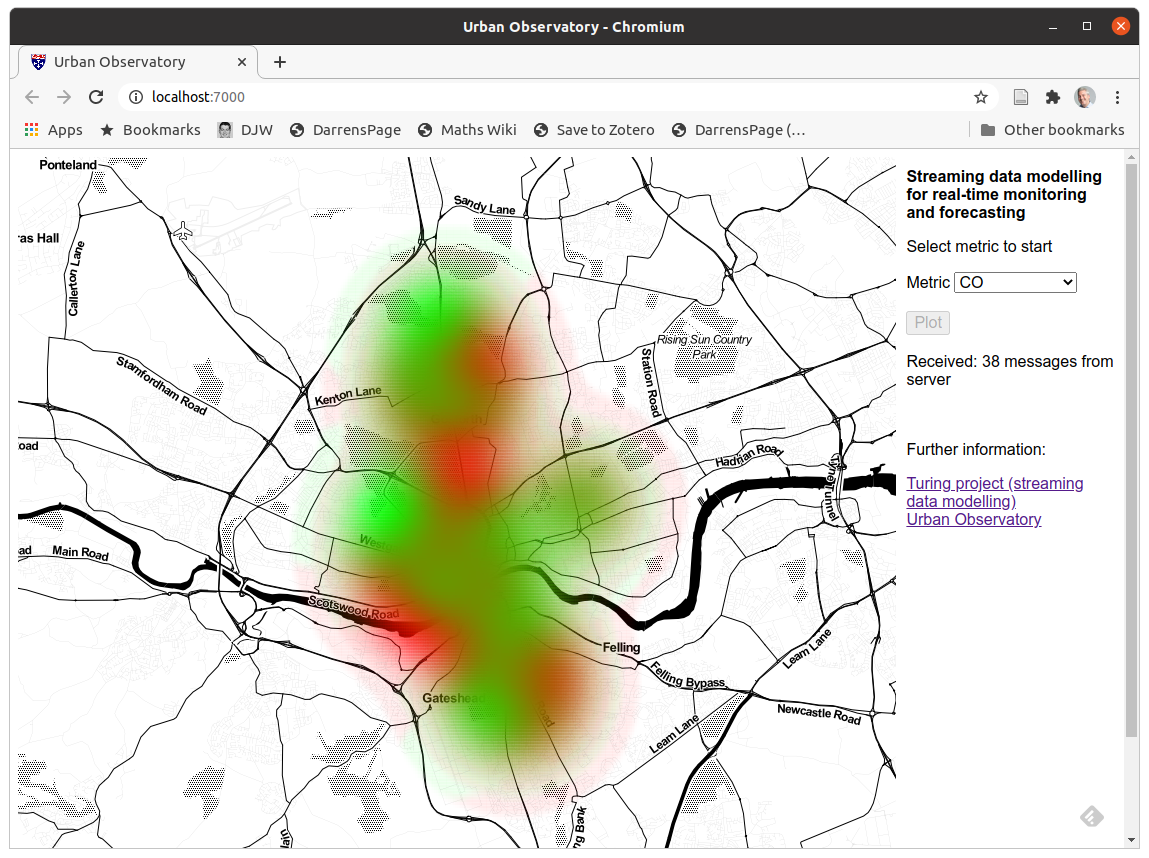
\includegraphics{uo-gui.png}
\caption{UO ``live'' monitoring}
\end{figure}

\end{frame}

\begin{frame}{Practical issues}
\protect\hypertarget{practical-issues}{}

\begin{itemize}
\tightlist
\item
  We have a running test-bed system that can visualise pollution levels
  across the city, using transparent fade-out to represent uncertainty
  in areas of poor sensor coverage, updating in real-time as each new
  observation arrives
\item
  Many practical issues requiring further work and collaboration with
  subject matter experts before public deployment
\item
  Modelling issues

  \begin{itemize}
  \tightlist
  \item
    Modelling sensor-specific issues and biases --- impact of biases on
    parameter inference --- especially length scales
  \item
    Incorporation of expert prior information
  \item
    Independent calibration and verification of maps, especially against
    areal data
  \end{itemize}
\item
  Visualisation issues

  \begin{itemize}
  \tightlist
  \item
    Colour-scales for inferred pollution levels
  \item
    Appropriate, calibrated visualisation of uncertainty
  \end{itemize}
\end{itemize}

\end{frame}

\begin{frame}{Current and future plans and projects}
\protect\hypertarget{current-and-future-plans-and-projects}{}

\begin{itemize}
\tightlist
\item
  Complete work on the air pollution case study
\item
  Neuroscience application
\item
  Engineering biology application
\item
  Complete rainfall modelling work
\item
  Collaboration on novel streaming data architectures
\item
  Further work on scalable sequential Bayesian updating methodology
\item
  Software for (functional) probabilistic programming on streaming data
\end{itemize}

\end{frame}

\end{comment}


\begin{frame}{Flood-PREPARED (NERC-funded)}
\protect\hypertarget{flood-prepared-nerc-funded}{}

\begin{block}{Predicting Rainfall Events by Physical Analytics of
REaltime Data}

\begin{itemize}
\tightlist
\item
  Real-time short-term high-resolution spatio-temporal rainfall
  modelling, synthesising \emph{areal} weather radar and \emph{point}
  rain gauge data
\item
  Near real-time emulation of and data assimilation for a hydrodynamic
  urban flood model
\item
  Hooked up to traffic monitors, CCTV feeds, social media sources, etc.,
  all live streaming (from the Urban Observatory), for the development
  of an emergency decision support system for Newcastle
\end{itemize}

\textbf{Johnson, Heaps, Wilson, W (2021)} Bayesian spatio-temporal model
for high-resolution short-term forecasting of precipitation fields,
\emph{arXiv}, 2105.03269

\end{block}

\end{frame}

\begin{frame}{Synthesising point and areal data (Flood-PREPARED)}
\protect\hypertarget{synthesising-point-and-areal-data-flood-prepared}{}

\begin{figure}
\centering
\includegraphics{ncl_z2_radar_grid_gauge.pdf}
\caption{Rainfall data}
\end{figure}

\end{frame}



\begin{frame}{Summary}
\protect\hypertarget{summary}{}

\begin{itemize}
\tightlist
\item
  The analysis and modelling of streaming data is becoming increasingly
  important
\item
  Typical motivations:

  \begin{enumerate}
  \tightlist
  \item
    Sequential analysis of ``live'' data in (near) real time
  \item
    Analysis of large data-sets based on ``one pass'' methods
  \item
    Parallel computation via stream \emph{splitting} and \emph{merging}
  \end{enumerate}
\item
  There exist computational models and software libraries for working
  with streaming data in an efficient and robust way
\item
  Functional (and reactive) programming languages and approaches are
  well-suited to working with (infinite) data streams (and probabilistic
  programs)
\item
  Time series are a natural fit to streaming data models, but not all
  streaming data applications have a natural temporal aspect
\item
  Many statistical models and algorithms can be adapted to a sequential
  context
\end{itemize}

\end{frame}
